\begin{problem}[Munkres \S52, Ex.\,2]
Let $\alpha$ be a path in $X$ from $x_0$ to $x_1$; let $\beta$ be
a path in $X$ from $x_1$ to $x_2$. Show that if
$\gamma=\alpha*\beta$, then $\hat\gamma=\hat\beta\circ\hat\alpha$.
\end{problem}
\begin{proof}
By Theorem 52.1, the paths $\alpha$ and $\beta$ induce a group homomorphism
$\hat\alpha\colon\pi_1(X,x_0)\to\pi_1(X,x_1)$ and
$\hat\beta\colon\pi_1(X,x_1)\to\pi_1(X,x_2)$, respectively. We want to
show therefore that the induced homomorphism
$\hat\gamma=\widehat{\alpha*\beta}$ is in fact equivalent to the
composition $\hat\beta\circ\hat\alpha$. Let $[f]$ be a loop based at $x_0$
then
\begin{align*}
\hat\gamma([f])&=\widehat{\alpha*\beta}([f])\\
               &=\bigl[\,\overline{\alpha*\beta}\,\bigr]*[f]*[\alpha*\beta]\\
               &=\bigl[\bar\beta*\bar\alpha\bigr]*[f]*[\alpha]*[\beta]\\
\shortintertext{by the well-definedness of the path product operation, we have}
               &=[\bar\beta]*[\bar\alpha]*[f]*[\alpha]*[\beta]\\
\shortintertext{by associativity of the path product,}
               &=[\bar\beta]*([\bar\alpha]*[f]*[\alpha])*[\beta]\\
               &=[\bar\beta]*\hat\alpha([f])*[\beta]\\
\shortintertext{where $\alpha([f])$ is a loop based at $x_1$ so}
               &=\hat\beta\left(\hat\alpha([f])\right)\\
               &=\bigl(\hat\beta\circ\hat\alpha\bigr)([f]).
\end{align*}
Thus, the following diagram commutes
\begin{center}
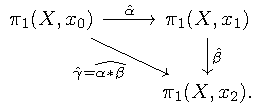
\includegraphics{figures/hw-10-pi-1-path-diagram}
\end{center}
\end{proof}
\newpage
\begin{problem}[Munkres \S52, Ex.\,3]
Let $x_0$ and $x_1$ be points of the path-connected space
$X$. Show that $\pi_1(X,x_0)$ is Abelian if and only if for every
pair $\alpha$ and $\beta$ of paths from $x_0$ to $x_1$, we have
$\hat\alpha=\hat\beta$.
\end{problem}
\begin{proof}
$\implies$ Let $f$ and $g$ be loops about $x_0$. Then, since $X$
is path-connected, we claim that $f$ and $g$ are homotopic to the
path product of two paths $\alpha$ and $\beta$ from $x_0$ to
$x_1$, say, $\alpha_1*\bar\beta_1$ and
$\alpha_2*\bar\beta_2$. More precisely, split $f$ into the path
$f_1=f(t/2)$ from $x_0$ to $x_2$ and $f_2=f((t+1)/2)$ from $x_2$
to $x_0$  and let $x_2$ be the point at $f(1/2)$. Then there
exists a path, say $\alpha$, from $x_2$ to $x_1$. Now we
construct the homotopy
\[H(x,t)=f_1(x/2)*\alpha(2tx)*\bar\alpha*((2t-1)x)*f_2((x+1)/2)\]
from $f=f_1*f_2$ to the loop $f=f_1*\alpha*\bar\alpha*f_2$.

$\impliedby$
\end{proof}
\newpage
\begin{problem}[Munkres \S52, Ex.\,4]
Let $A\subset X$; suppose $r\colon X\to A$ is continuous map such
that $r(a)=a$ for each $a\in A$. (The map $r$ is called a
\emph{retraction} of $X$ onto $A$.) If $a_0\in A$, show that
\[
r_*\colon\pi_1(X,x_0)\longrightarrow\pi_1(A,a_0)
\]
is surjective.
\end{problem}
\begin{proof}
\end{proof}
\newpage
\begin{problem}[Munkres \S53, Ex.\,6]
Show that if $X$ is path connected, the homomorphism induced by a
continuous map is independent of the base point, up to
isomorphisms of the groups involved. More precisely, let $h\colon
X\to Y$ be continuous, with $h(x_0)=y_0$ and $h(x_1)=y_1$. Let
$\alpha$ be a path in $X$ from $x_0$ to $x_1$, and let
$\beta=h\circ\alpha$. Show that
\[
\hat\beta\circ(h_{x_0})_*=(h_{x_1})\circ\hat\alpha.
\]
This equation expresses the fact that the following diagram of
maps ``commutes''
\begin{center}
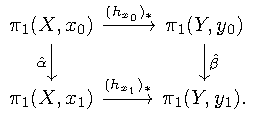
\includegraphics{figures/hw-10-path-connected-hom-indep}
\end{center}
\end{problem}
\begin{proof}
\end{proof}
\newpage
\begin{problem}[Munkres \S55, Ex.\,1]
Show that if $A$ is a retract of $B^2$, then every continuous map
$f\colon A\to A$ has a fixed point.
\end{problem}
\begin{proof}
\end{proof}
\newpage
\begin{problem}[Munkres \S55, Ex.\,2]
Show that if $h\colon S^1\to S^1$ is nulhomotopic, then $h$ has a
fixed point and $h$ maps some point $x$ to its antipode $-x$.
\end{problem}
\begin{proof}
\end{proof}
\newpage
\begin{problem}[(A)]
Prove that every $m$-manifold is locally path-connected.
\end{problem}
\begin{proof}
\end{proof}
\newpage
\begin{problem}[(B)]
Prove that every $m$-manifold is regular.
\end{problem}
\begin{proof}
\end{proof}
\newpage
\begin{problem}[(C)]
Prove that there is no $1$-$1$ continuous function $\iota\colon
S^1\to\RR$. You may assume any fact about trigonometric
functions. (Note: this shows in particular that there is no
$\iota\colon S^1\to\RR$ with $p\circ\iota$ equal to the identity
map, where $p$ is the map in the note on the Fundamental Group of
the Circle.)
\end{problem}
\begin{proof}
\end{proof}
\newpage
\begin{problem}[(D)]
Prove Proposition C from the note on the Fundamental Group of the Circle.
\end{problem}
\begin{proof}
\end{proof}

%%% Local Variables:
%%% mode: latex
%%% TeX-master: "../MA571-HW-Current"
%%% End:
